\chapter{Implementation} \label{sec:implementation}
\section{Platform}
We choose a C++ language for implementing our solutions, because we need low level code optimization and features like SIMD instructions, which are not available in other languages. Even if the CUDA is developed to work with multiple languages, cooperation with  C++ is one of the best, because also CUDA kernels are written in C++. Also platform independence of C++ is useful because we developed programs on Windows and than run on Linux clusters.

\section{K-means algorithm} \label{sec:kMeansAlgorithm}

As we can see in serial implementation~\autoref{lst:kMeansCode}, there are many cycles dependent on data size, so with growing number of data, serial version comes much slower. For example in two nested cycles on lines \autoref{lst:nestedCyclesBegin}-\autoref{lst:nestedCyclesEnd} of \autoref{lst:kMeansCode}, slowdown is great and this part of code is good target for parallelization.\\

\begin{lstlisting}[caption={k-means algorithm}, language=C++, escapeinside={\%*}{*)}, label={lst:kMeansCode}, numbers=left]
CreateLSH(width, hashTablesCount, basicHashFunctions)
{
  // Main iteration loop
  for( i = 0; i < iterationsCount; i++)
  {
    assign_to_clusters(data, means);
    compute_means(data_means);
  }
}

// Assign points to clusters
%*\label{lst:assignToClusters}*)assign_to_clusters(data, means)
{
//Iterate through data
%*\label{lst:nestedCyclesBegin}*)  for( d = 0; d < data_size; d++)
  {
    assigned_cluster = 0;
    min_distance = MAX_VALUE;
// Iterate through means
    for( m = 0; m < means_size; m++)
    {
      distance = count_distance( data[d], means[m] );
// If m-cluster is closer, reassign cluster
      if ( distance < min_distance )
      {
        assigned_cluster = m;
        min_distance = distance;
      }
    }
    data[d]->assigned_cluster = assigned_cluster;
%*\label{lst:nestedCyclesEnd}*)  }
}

// Compute new means
%*\label{lst:computeNewMeans}*)compute_means(data, means)
{
// Create new means array, all values are set to 0
  for( m = 0; m < means_size; m++)
  {
    new_means.push_back(new mean(0));
  }
  
// Iterate through data and accumulate data in appropriate new mean
  for( d = 0; d < data_size; d++)
  {
    assigned_cluster = data[d]->assigned_cluster;
    new_means[assigned_cluster]->contained_points++;
    for( dim = 0; dim < dimensions; dim++)
    {
      new_means[assigned_cluster]->coordinates[dim] +=
        data[d]->coordinates[dim];
    }
  }
  
// Count new means coordinates (arithmetic mean)
  for( m = 0; m < means_size; m++)
  {
    for( dim = 0; dim < dimensions; dim++)
    {
      new_means[m]->coordinates[dim] /=
        new_means[m]->contained_points;
    }
  }
}

// Function for counting distance
count_distance(point, mean)
{
  sum_squares = 0;
  for( dim = 0; dim < dimensions; dim++)
  {
    difference = point->coordinates[dim] - mean->coordinates[dim];
    sum_squares += difference * difference;
  }
  return sqrt( sum_squares );
}
\end{lstlisting}

\section{Parallelization}
As we mentioned in \autoref{sec:kMeansAlgorithm}, classical k-means algorithm contains many compute-intensive cycles, which could be parallelized. Problem is that the algorithm contains some compute dependencies, for example parallelization of nested cycles on lines \autoref{lst:nestedCyclesBegin}-\autoref{lst:nestedCyclesEnd} of \autoref{lst:kMeansCode} is problematic, because we need to accumulate coordinates in shared variable. These dependencies must be solved some way for correct parallelization.

\subsection{CPU versions}
We tried to used the most modern technologies offered by the newest CPU architectures to speed up k-means algorithm by parallelization. We created two levels of parallelization, first based on thread level (using more logical cores on single CPU) and than vectorization level using SIMD instructions.

\subsubsection{Thread level parallelization}
For thread level parallelization, we choose Threading Building Blocks (TBB) library from Intel. This library offers algorithms and data structures for parallel programing using multi-core processors but relieve programmer from complications arising from the use of native threading packages and handling particular threads. Manual thread creation, execution, synchronization and termination is hidden by using by creating TBB tasks which are processed on individual cores dynamically by the library. Also efficient use of CPU caches is automated.\\
We reworked program so points are split in groups, each group forming one TBB task.\\
\begin{description}
\item[Assigning to clusters]The first part of algorithm, assigning to clusters~\autoref{lst:kMeansCode},~\autoref{lst:assignToClusters}, is not so problematic, because only write operation is assigning cluster to point. Each point is contained in one and only one TBB task, which is processed by single thread, so it could not be read or written from other threads.\\
Second possible solution is to split means into groups and parallelize algorithm by tasks containing means. This solution is significantly slower, because we must synchronize writing information to each point about assigned cluster. If we want to remember this information in means (by accumulating assigned points to each mean) we hit a problem, because after assigning point to mean, we could not know if other mean is not closer to processed point so this way o parallelization is too computationally intensive.\\
\item[Compute new means]The second part of the algorithm, counting new means~\autoref{lst:kMeansCode},~\autoref{lst:computeNewMeans}, is more problematic, because we approach means from different TBB tasks, so accumulating of coordinates must be synchronized. We solved this problem by local copy of means in each TBB task, so we avoided the collisions. For joining tasks, we used TBB reduce algorithm, when to tasks are joined, local arrays of means coordinate sums are correctly added.\\
Also in this part of algorithm exists second possible solution by approaching parallelization by splitting means. This is more compute intensive because in this solution, for each mean, we must iterate through all points and accumulate coordinates but in previous solution, we iterate only through points and than, we join single tasks which takes logarithmic time depends on number of tasks.
\end{description}
Because both tasks are parallelized by same approach (splitting points to tasks, not the means), we joined both steps into one~\autoref{fig:computeflow} and gain more speed up because of omitting one start and one finish of TBB parallel task which has big overhead.
\begin{figure}[h]
  \centering
  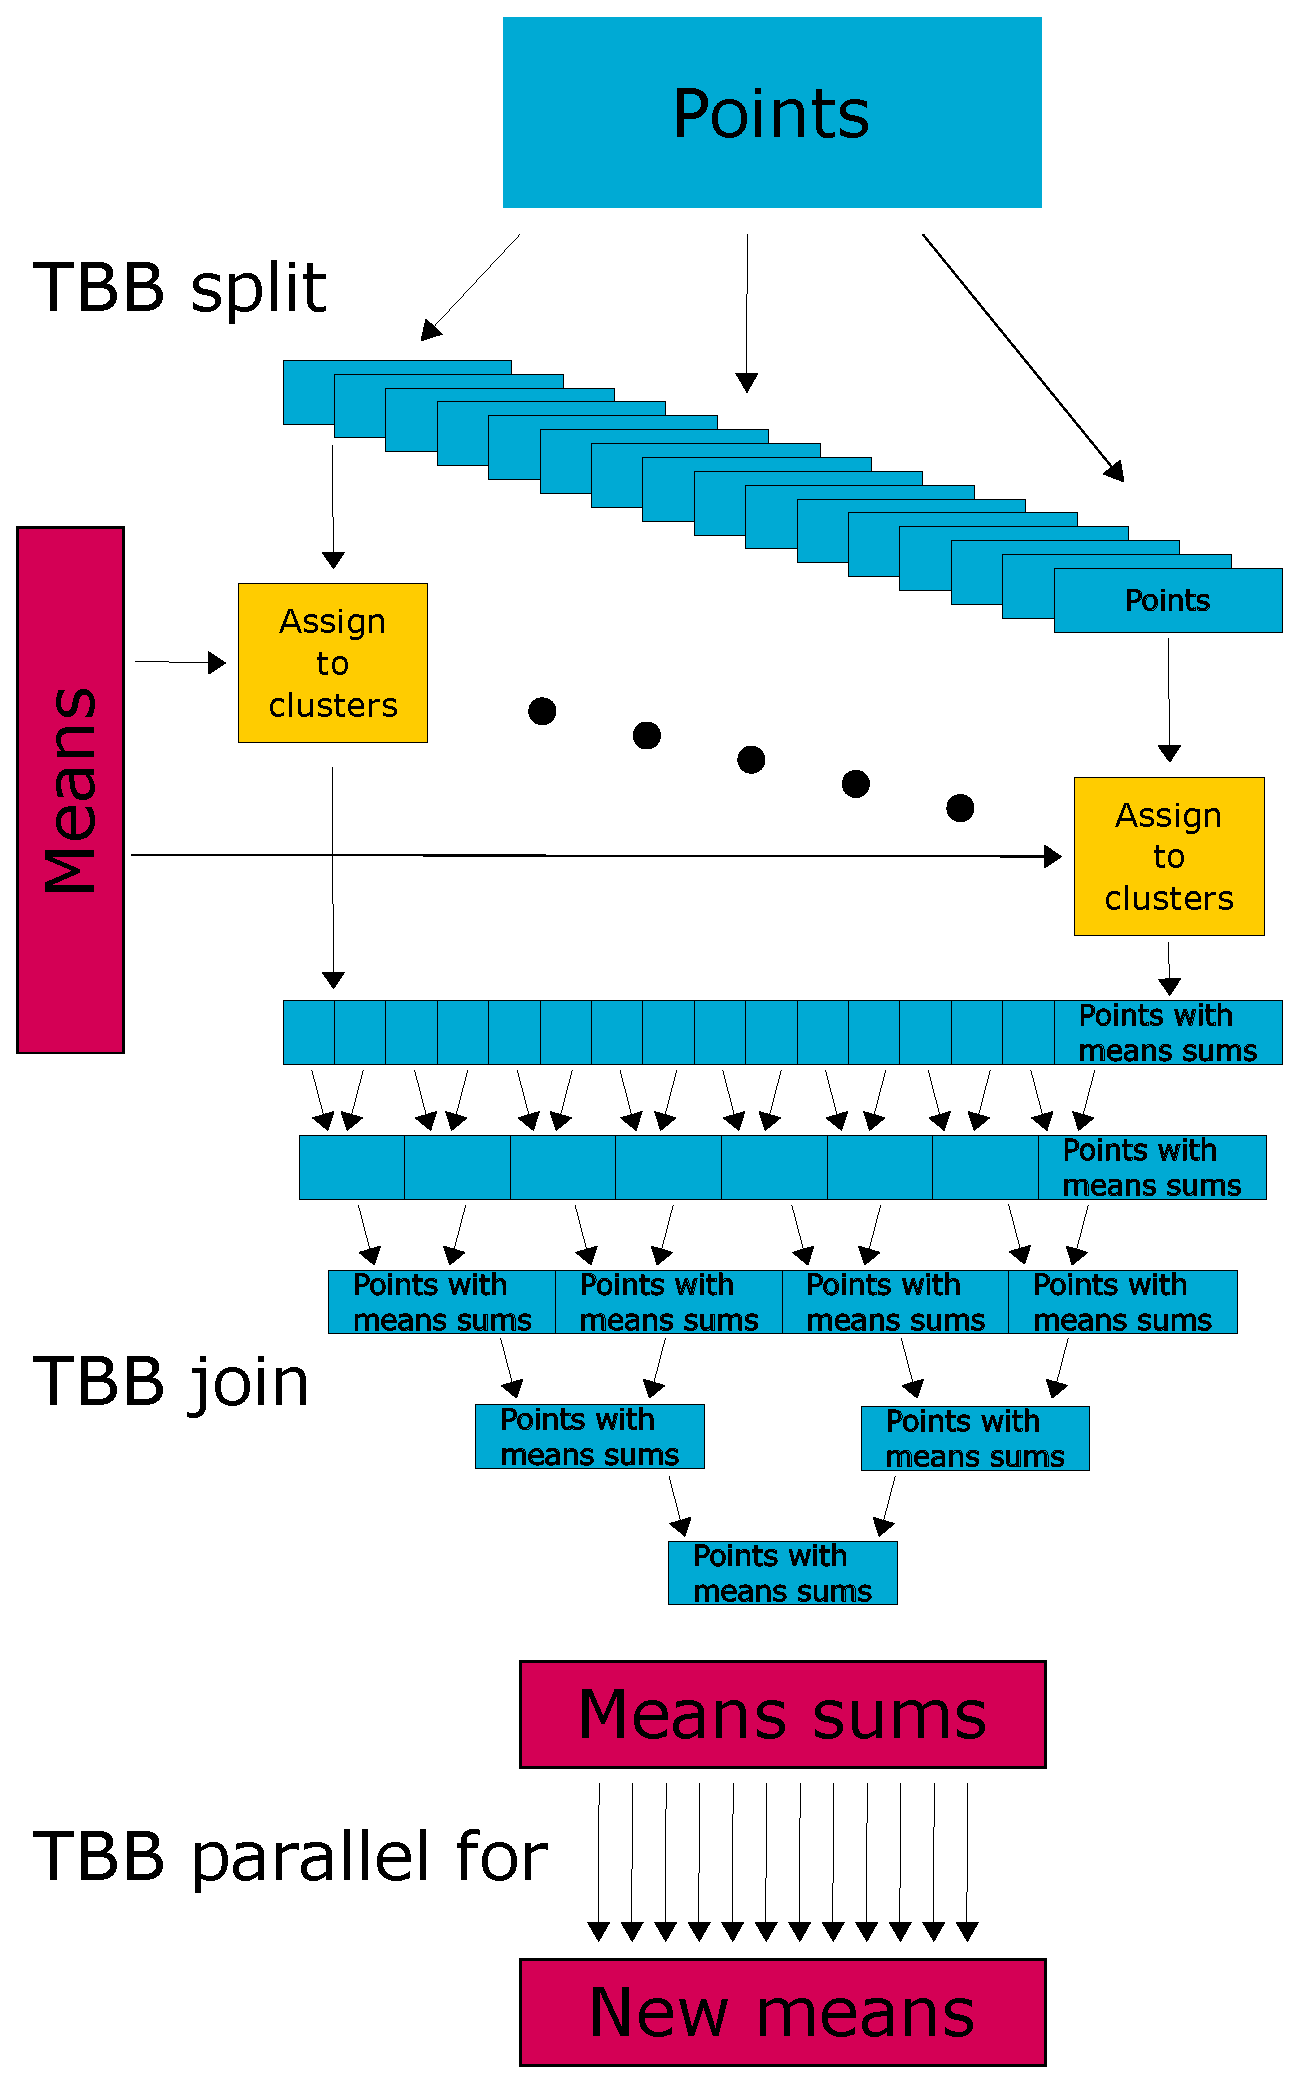
\includegraphics[width=1\linewidth]{img/computeFlow.eps}
  \caption{Compute flow}
  \label{fig:computeflow}
\end{figure}
\subsubsection{Vectorization}
For additional speed-up, we decided to use Simple instruction, multiple data (SIMD) as second layer of parallelization, concretely Streaming SIMD instructions (SSE), which are extension of x86 architecture. These instructions could greatly speed up the computation when exactly the same operations are performed on multiple data objects. Because points are already parallelized by TBB, we use SIMD inductions to parallelize smaller cycles iterating through dimensions, which are very often used in the algorithm. This cycle is usually much smaller (up to number of dimensions) than data but contains only few instructions which is precisely suitable for usage of SSE instructions so the loops will be up to four times faster (depend on number of dimensions) than non-SSE version.
\clearpage
\subsection{GPU versions}
For maximum speedup of this algorithm, we implemented versions using GPU, which offers hundreds of cores, so speed up of algorithm should be more than ten times better than parallel CPU version. Because of GPU architecture special features and the wide diversity of the input data, we developed more algorithm versions to reflect this particularities.\\
Also on GPU architecture we could divide algorithm to two layer of parallelization, using CUDA characteristics, because work on this platform is divided into blocks and each block is than executed by multiple threads. Because number of threads in single block is significantly bigger than possible count of instructions executed in parallel using SIMD, we decided to use different approach and use the thread layer in same way as the block layer, so both layers parallelize the task in terms of points.
Because the GPU compute effectiveness very depends on using different types of memory and the efficiency of its usage, it really depends on algorithm design. This problem is difficult to solve by single algorithm, because we need to use the data input characteristics. Here are some possibilities of data variety:
\begin{description}
\item[Big data] The first but maybe the biggest problem is the size of points. Because the input data are limited only by computer, so most often by host data storage, it can easily happen that the input data will not fit into the device biggest memory - global memory. Because this problem is also limiting on nonGPU versions, we have only focused on case when data fits in standardly the biggest memory on host - the RAM memory.
\item[Many dimensions] Other data problem could be many dimensions of the input space. Because basic GPU algorithm works similar as CPU version but without SIMD instructions, each thread in block must iterate through all dimensions which could be done better especially when the input data contains only few points.
\item[Few means] Opposite data attribute could be only few means. Than we could make several copies to fill in memory and avoid possible collisions. Problem is that we must join all copies onto so making so many copies is not so efficient.
\end{description}

The main problem is data size (both points and means) ín compare to memory size. In \autoref{tab:datamemoryfilling} is solution for each case when the appropriate data will not fit to the appropriate memory.

\newcolumntype{Y}{>{\RaggedRight\arraybackslash}X} 
\def\tabularxcolumn#1{m{#1}}
\begin{table}[h]
\centering
\caption{Data sizes and memory filling}
\label{tab:datamemoryfilling}
\begin{tabularx}{\textwidth}{|r|Y|Y|}
\cline{1-3}
\rowcolor[HTML]{AAD400} 
&Means&Points\\ \cline{1-3}
{\cellcolor[HTML]{AAD400}} Local memory&We could  share means between threads in Grid and store them in Shared memory.& Points are usually too bigger to fit in Local Memory, if so, we could place them into constant memory.\\ \cline{1-3}
{\cellcolor[HTML]{AAD400}} Shared memory&If means could not fit into Shared Memory, we could split them into more groups and make more iterations each only with means part.&Points sometimes could fit in Shared memory, if so, we could speed up the computation.\\ \cline{1-3}
{\cellcolor[HTML]{AAD400}} Global memory&If means does not fit even in Global memory on device, we must iterate through them, but this case usually does not occur.& When points are bigger than Global memory, we must swap appropriate part of them on device.\\ \cline{1-3}
\end{tabularx}
\end{table}

\subsubsection{Basic version}~\label{sssec:basicversion}
We have started with implementation of basic version, where we suppose that all data fits in device global memory. This implementation uses two CUDA kernels, first of them only find nearest cluster (\autoref{lst:findNearestClusterKernel} of \autoref{lst:simplekernel}). Each thread in block process one point by simple iterating through all means and dimensions. Number of threads in depends on SM capability of hardware. Number of blocks is simply the ceiling of number of points divided by number of threads per block. In this basic version, all data are stored in global memory and only memory caching is used for better memory latency. \\
Second task of this basic version is to count new means (\autoref{lst:countNewMeansKernel} of \autoref{lst:simplekernel}). In this kernel, each thread handles one mean. It iterates through all points and if point is assigned to appropriate mean, algorithm accumulates its coordinates. After all points are processed, new means are counted from accumulated sums by division by assigned points.\\
\\
\textcolor{red}{Add image with basic compute flow on CUDA?}
\\
\begin{lstlisting}[caption={CUDA simple kernel}, language=C++, escapeinside={\%*}{*)}, label={lst:simplekernel}, numbers=left]
%*\label{lst:findNearestClusterKernel}*)findNearestClusterKernel
  (meansSize, means[], dataSize, data[]
  , assignedClusters[], dimension)
{
  id = threadIdx.x + blockIdx.x * blockDim.x;
  minDistance = LLONG_MAX, distance = 0, difference = 0;
  for ( i = 0; i < meansSize; ++i )
  {
    distance = 0;
    for ( j = 0; j < dimension; ++j )
    {
      difference =
        means[ i * dimension + j ]
        - data[ id * dimension + j ];
      distance += difference * difference;
    }
    if (minDistance > distance)
    {
      minDistance = distance;
      assignedClusters[id] = i;
    }
  }
}


%*\label{lst:countNewMeansKernel}*)countNewMeansKernel
  (assignedClusters [], dataSize
  , data[], means[], dimension)
{
    id = threadIdx.x + blockIdx.x * blockDim.x;
    idOffset = id * dimension;
    count = 0;
    for ( i = idOffset; i < idOffset + dimension; ++i )
    {
        means[i] = 0;
    }
  %*\label{lst:bigdataloop}*)  for ( i = 0; i < dataSize; ++i )
    {
        if ( assignedClusters[i] == id )
        {
            for ( j = 0; j < dimension; ++j )
            {
                means[idOffset + j] +=
                  data[i * dimension + j];
            }
            ++count;
        }
    }
    for ( i = idOffset; i < idOffset + dimension; ++i )
    {
        means[i] /= count;
    }
}
\end{lstlisting}

\subsubsection{Atomic operations}
Because of huge slow down in the basic version~\autoref{sssec:basicversion} in counting new means from assigned clusters, we need to iterate through tens of thousands of points~(\autoref{lst:bigdataloop} in \autoref{lst:simplekernel})  and only if we hit point assigned to appropriate cluster, we accumulate its coordinates. This is because we could not accumulate these in find nearest cluster function (\autoref{lst:findNearestClusterKernel}), because we could get several race conditions when writing from many threads to single cluster. If we solved this problem, than second step of the algorithm could be only to divide accumulated coordinate sums by number of assigned cluster and avoid time-consuming loop through every point. This race conditions could be solved by atomic operations, which could easily protect accumulating of coordinates and avoid this problem, but atomic operations have some overhead and when we have only few means, this overhead causes a big algorithm slow down so in this case, this problem must be solved in some other way.

\subsubsection{Many dimensions problem}~\label{sssec:manyDims}
Because in basic version, each point is processed by single thread, kernel run could become slower when the dimension of input space is big. Like in CPU version with SIMD, we implemented a version which simulate SSE instructions so if the dimension of space is big enough, we launch thread block for each point and threads in these block works like SIMD and iterate through dimensions. Each thread has its local sum of distances in each dimension so than we need to add these values from each thread. Because these values must be accessible from all threads in warp, we used shared memory.\\
This could be solved by many ways so we tried to optimize this process for CUDA environment.\\
\\
\textcolor{red}{Add images of compute flow in each type of reduction?}
\\
\begin{description}
\item[Interleaved addressing] In this access, we reduce the partial sums in array of size $N$ iteratively. In each step, we need only half of a array from previous step, so in first step ($i=1$), we start $N/(i^2)$ threads, each thread access only partial sums on positions dividable by $2^i$, add partial sum from position $2^{(i-1)}$ bigger and store the value.
\begin{lstlisting}
for ( stride=1; stride < threadsInBlock; stride*=2)
{
  if (threadID % ( 2 * stride ) == 0)
  {
    sums[threadID] += sums[threadID + stride];
  }
  __syncthreads();
}
\end{lstlisting}
Main problem of this solution is that modulo operator is very slow and that in highly divergent warps, reduction is very inefficient.
\item[Interleaved addressing 2]This solution is similar to previous but we removed problems of first solution. At first, we removed the modulo operation and second thing is that in each we used only threads with IDs less than half of array size from previous step. 
\begin{lstlisting}
for ( stride=1; stride < threadsInBlock; stride*=2)
{  i = 2 * stride * threadID;
  if ( i < threadsInBlock)
  {
    sums[index] += sums[index + stride];
  }
  __syncthreads();
}
\end{lstlisting}
Because we using shared memory for sums, we hit a new problem, bank conflicts, so we must use little bit different approach if we need to solve this.
\item[Sequential addressing]Problem with bank conflicts could be solved by using reverse loop and different type of addressing. In this solution we used same threads as in previous solution, but we access only items on the front of the array. This means that we again start with half of threads than array size but each thread takes item from array with same id as thread id and sums it with item with id $threadID + stride$. This means that the actual partial sums in each step is in the front of the array so we have avoided bank conflicts.
\begin{lstlisting}
for ( stride=threadsInBlock; stride > 0; stride>>=1)
{
  if ( threadID < stride )
  {
    sums[threadID] += sums[threadID + stride];
  }
  __syncthreads();
}
\end{lstlisting}
Even in this solution we have problem with unused threads. In first iteration, half of them is unused, in second iteration, only a quarter of all threads working etc. This could be partially solved by making first step when loading data to share memory, so we need only half of all threads or in other words, we could process twice the data volume than without this improvement.
\item[Unrolling loop]Because we could select the number of threads in block, we could choose same number as number of cores in SM and because instructions are SIMD synchronous within warp, we do not need thread synchronization $syncthreads()$ and because we know the block size at the compile time, we could template this method so big part of work will be resolved in compile time.
\begin{lstlisting}
if (threadIdx.x < blockDim.x / 2)
  {
    if (blockSize >= 64) distances[threadId] +=
      distances[threadId + 32];
    if (blockSize >= 32) distances[threadId] +=
      distances[threadId + 16];
    if (blockSize >= 16) distances[threadId] +=
      distances[threadId + 8];
    if (blockSize >= 8) distances[threadId] +=
      distances[threadId + 4];
    if (blockSize >= 4) distances[threadId] +=
      distances[threadId + 2];
    if (blockSize >= 2) distances[threadId] +=
      distances[threadId + 1];
  }
\end{lstlisting}
\item[Shuffle instructions]From Compute capability 3.0, we could use special shuffle instructions. These instructions was designed for cooperation between threads in one warp and to thread process local data in warp scope. Usually when we need to exchange data between threads in warp, we are forced to use shared memory, because we can't access local memory from other thread and this is exactly what shuffle instructions resolving. When we use shuffle instructions, we could use only the local memory which is significantly lower latency and higher bandwidth than shared memory and in addition shuffle instructions are faster than instructions on shared memory - single instruction versus three on shared memory (write, synchronize, read). So when we use shuffle instructions for sum partial sums, we gain additional speed up (but only CC 3.0 and newer).
\end{description}

\subsubsection{Few means}
When we need to compute only few means, we could solve problems with conflicts by making local copies of all means sums in shared memory and than merge it in similar way as in~\autoref{sssec:manyDims}.\\
Each thread have its copy of means and shares it with only few other threads so we reduce conflicts by number of means copies. As an extreme case, every thread could have its own copy of means sums so we can completely avoid collisions. Problem is that we must merge all copies in next step, so we must select between number of collisions and merge demands.
Because merging of means copies is harder than merging distances (we don't merge all data into single value but we need to sum only corresponding data. Also the amount of data is many times bigger.\\
We also implemented solution for case when means closely do not fit in shared memory. Than we could split means and counts only with part of means and than compute the same task but with other part of means. Also this problem requires post processing because all points are assigned two more means (from each part we choose the nearest mean) so we need to choose the nearest means and than accumulate coordinates sums. Because post processing in this solution is harder, it makes sense only for small number of means parts.

\subsubsection{Big data}
Problem with big data is obvious because points could not fit in device memory. This could be solved by split data into smaller parts so we can fit two parts at once in global memory.Because on CUDA has capability to transfer data and process other data at once, we can work on one part which is already transfered on device while other chunk of points is transfered onto device.
Than we must compute new means but because we expect that means fit in device memory, we could use same function as in other solutions.

\section{??Tools??}
\subsection{??Data generation??}
\subsection{??Result validation??}